\documentclass[red]{beamer}
\usetheme{CambridgeUS}
\setbeamertemplate{navigation symbols}{}
\setbeamertemplate{footline}{}
\setbeamertemplate{items}[triangle] 
\renewcommand{\footnoterule}{}

\usepackage[utf8]{inputenc}
\usepackage[slovak]{babel}
\usepackage[IL2]{fontenc}
\usepackage[protrusion=true,expansion=true]{microtype}
\usepackage[none]{hyphenat}

\usepackage{hyperref}
\urlstyle{same}
\usepackage{textcomp}
\usepackage{xargs}
\usepackage{graphicx}
\usepackage{wrapfig}
\usepackage[absolute,overlay]{textpos}
\usepackage{amssymb}
\usepackage{amsmath}
\usepackage{verbatim}
\usepackage{eurosym}

\newcommand{\TODO}{{\color{red}!!!!!!!!!!!!!!!!!!!!!!!!}}
\newcommand{\vlnovka}{\raise.35ex\hbox{$\scriptstyle\mathtt{\sim}$}}

\newcommandx{\odrazka}[3][1=1, 2]{\begin{itemize}\item<#1-#2> #3\end{itemize}}



%%%%%%%%%%%%%%%%%%%%%%%%%%%%%%%%%%%%%%%%%%%%%%%%%%

\begin{document}

\large

\title{Odstraňovanie tieňov}
\subtitle{Spracovanie farebného obrazu}
\author{Rastislav Kamenický, Michal Piovarči, Matej Kopernický}
\date{14.5.2013}

{
\setbeamertemplate{background canvas}{
\includegraphics[width=\paperwidth,height=\paperheight]{title}}
\begin{frame}[plain,t]
\begin{center}
\color{white}
\vspace{2,5cm}
\huge\inserttitle\\
\vspace{0.9cm}
\Large\insertsubtitle\\
\vspace{1.75cm}
\color{black}
\large\insertauthor\\
\bigskip\bigskip
\href{http://www.github.com/misop/shadow_removal}{github.com/misop/shadow\_removal}
\end{center}
\end{frame}
}



\begin{frame}
\begin{columns}
\begin{column}{0.59\textwidth}
\odrazka[1]{Široké využitie pri úprave fotografií}
\odrazka[2]{Neexistuje žiadne 100\% riešenie}
\odrazka[3]{Väčšinou sú vyžadované parametre snímacieho zariadenia, vlastnosti scény a pod.}
\odrazka[4]{Cieľ -- vytvoriť jednoduchú metódu, ktorej vstupom je len obrázok a je potrebné len minimum interakcie}
\end{column}
\begin{column}{0.4\textwidth}
\uncover<1->{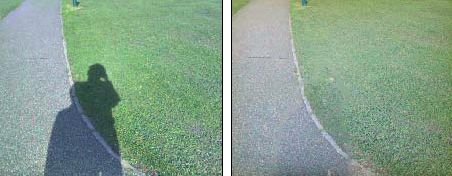
\includegraphics[width=\linewidth]{./img/1.jpg}}\\
\bigskip
\uncover<1->{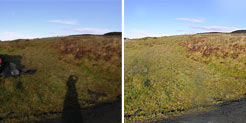
\includegraphics[width=\linewidth]{./img/2.jpg}}
\end{column}
\end{columns}
\end{frame}





\end{document}